% !TeX root = document.tex
% !TeX encoding = UTF-8 Unicode

\section{Time-Scale Systems}%
\label{sec:ts-systems}

\subsection{Time Scale Calculus}%
\label{subsec:ts-calculus}

\begin{slide}{Time-Scale Calculus}
  \begin{columns}[c]
    \begin{column}{0.48\textwidth}
      \begin{itemize}
        \item Unifies the continuous- and discrete-time calculi.
        \item Uses the so-called delta-derivative (\(\Delta\)-derivative).
        \item Exists for different time-sets, not only the continuous and
              discrete case.
      \end{itemize}
      \begin{figure}[ht!]
        \centering
        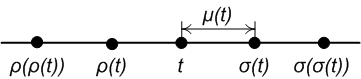
\includegraphics[width=0.6\linewidth]{ts-jump}
        \caption{Time-Scale jump operators. Source: \url{https://shorturl.at/bcJY1}}%
      \end{figure}
    \end{column}%
    \hfill%
    \begin{column}{0.48\textwidth}
      \begin{equation}
        \mathbb{T} = h\mathbb{Z} | \mathbb{R} | \mathbb{T}_{\textrm{iso}}
      \end{equation}
      %
      \begin{align}
        \textrm{forward:~}  & \sigma(t) = \inf\{\tau\in\mathbb{T}|\tau>t\}, \\
        \textrm{backward:~} & \rho(t) = \sup\{\tau\in\mathbb{T}|\tau<t\}.
      \end{align}
      %
      \begin{equation}
        \mu(t) = \sigma(t)-t \leftarrow \textrm{graininess}
      \end{equation}
      %
      \begin{equation}
        f(\sigma(t)) = f(t) + \mu(t)f^{\Delta}(t).
      \end{equation}
      %
      \begin{equation}
        f^{\Delta}(t) = \lim_{\delta\rightarrow{}\mu(t)}\frac{f(t+\delta)-f(t)}{\delta}.
      \end{equation}
    \end{column}%
  \end{columns}
\end{slide}

\begin{slide}{Time-Scale System}
  \begin{columns}[c]
    \begin{column}{0.38\textwidth}
      \begin{itemize}
        \item Allows to evolve the system with arbitrary sampling-times.
        \item Has it own stability criteria based on the Hilger's circle.
      \end{itemize}
    \end{column}%
    \hfill%
    \begin{column}{0.58\textwidth}
      \begin{align}
        \textrm{Continuous-Time System} & \nonumber                                                                 \\
        \dot{x}(t)                      & = \mathcal{A}x(t) + \mathcal{B}u(t),                                      \\
        y(t)                            & = Cx(t) + Du(t),                                                          \\
        \textrm{Time-Scale System}      & \nonumber                                                                 \\
        x^{\Delta}(t)                   & = A(\mu(t))x(t) + B(\mu(t))u(t),                                          \\
        y(t)                            & = Cx(t) + Du(t),                                                          \\
        \phantom{1}                     & \phantom{1}                                 \nonumber                     \\
        A(\mu(t))                       & = \frac{e^{\mathcal{A}\mu(t)}-I}{\mu(t)},                                 \\
        B(\mu(t))                       & = \int_{0}^{\mu(t)}\frac{e^{(\mu(t)-s)\mathcal{A}}}{\mu(t)}\mathcal{B}ds.
      \end{align}
    \end{column}%
  \end{columns}
\end{slide}

\begin{slide}{Stability Criteria}
  \begin{columns}[c]
    \begin{column}{0.48\textwidth}
      The system is stable if all of it's poles are within the Hilger's circle,
      defined as a the circle centered at \((-\frac{1}{\mu}, 0)\) and with
      radius \(\frac{1}{\mu}\).

      Note that the circle changes with the sampling-time (\(\mu\)).

      \begin{equation}
        \mathcal{H}_{\mu} \coloneqq \left\{ z \in \mathbb{C} : \abs{z + \frac{1}{\mu}} < \frac{1}{\mu} \right\}
      \end{equation}
    \end{column}%
    \hfill%
    \begin{column}{0.48\textwidth}
      \begin{figure}[ht!]
        \centering
        \resizebox{\linewidth}{!}{%
          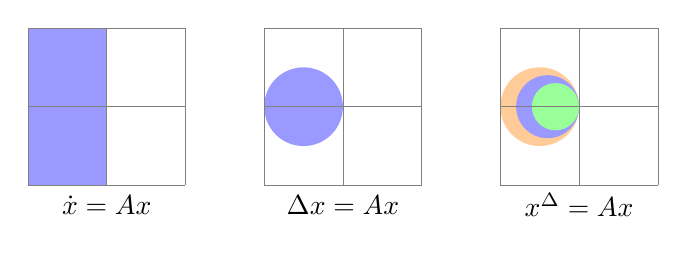
\begin{tikzpicture}
            \fill [blue!40!white]           (0, 0) rectangle (1, 2);
            \draw [step=1cm,gray,very thin] (0, 0) grid      (2, 2);
            \node at (1, -0.25) {\(\dot{x}=Ax\)};

            \fill [blue!40!white]           (3.5, 1) circle (0.5);
            \draw [step=1cm,gray,very thin] (3, 0)   grid   (5, 2);
            \node at (4, -0.25) {\(\Delta{}x=Ax\)};

            \fill [orange!40!white]         (6.5, 1) circle (0.5);
            \fill [blue!40!white]           (6.6, 1) circle (0.4);
            \fill [green!40!white]          (6.7, 1) circle (0.3);
            \draw [step=1cm,gray,very thin] (6, 0)   grid   (8, 2);
            \node at (7, -0.25) {\(x^{\Delta{}}=Ax\)};
          \end{tikzpicture}%
        }
        \caption{Different stability regions}%
      \end{figure}
    \end{column}%
  \end{columns}
\end{slide}
